\documentclass[tikz,border=4pt,11pt]{standalone}
\usepackage{amsmath}
\definecolor{ink}{RGB}{42,52,64}
\definecolor{first}{RGB}{146,79,26}
\definecolor{second}{RGB}{26,99,111}
\definecolor{areacell}{RGB}{232,232,232}

% The Dyck path with area sequence (0,1,2,2,3).
% Left: the cells (i,c), i<c, of the board (3,5,5,5,5), i.e. the edges of the
%   unit interval graph.  The rows 1 and 2, where a peak interval starts, are
%   coloured; they form the skew shape (3,2) after shifting row k left by k.
% Middle: the tableau of shape (3,2) with rows 124 and 35.
% Right: the corresponding particle hops.  Particle 1 starts at 1 and ends at
%   3, particle 2 starts at 2 and ends at 5; entry t of the tableau is the t-th
%   hop.  The hop at time 4 moves a particle to the right of the previous one,
%   giving the natural descent 3.

\begin{document}
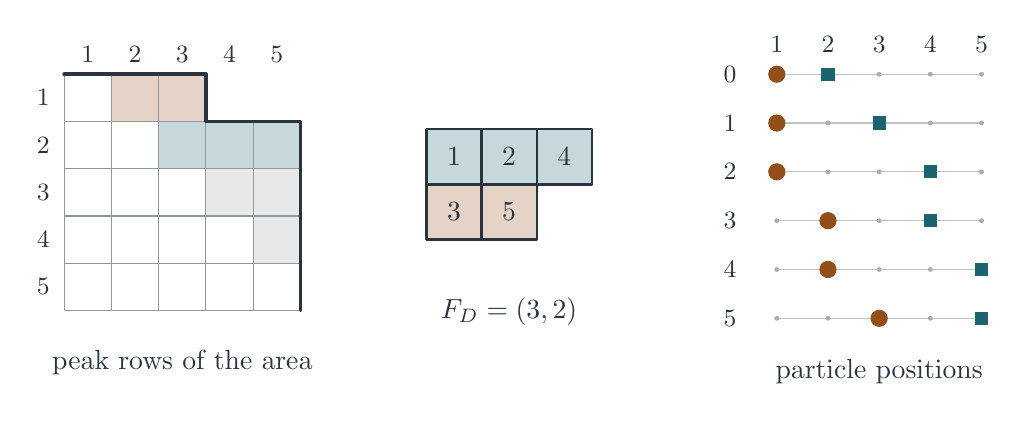
\begin{tikzpicture}[text=ink,line cap=round,line join=round,
  p1/.style={circle,fill=first,inner sep=2.2pt},
  p2/.style={rectangle,fill=second,inner sep=2.4pt}]

% ---------- area cells of the board ----------
\begin{scope}[x=.6cm,y=.6cm]
  \def\lam{{3,5,5,5,5}}
  \foreach \i in {1,...,5} {
    \pgfmathtruncatemacro{\L}{\lam[\i-1]}
    \foreach \c in {1,...,\L} {
      \ifnum\c>\i
        \ifnum\i=1 \fill[first!25] (\c-1,-\i) rectangle (\c,-\i+1);
        \else\ifnum\i=2 \fill[second!25] (\c-1,-\i) rectangle (\c,-\i+1);
        \else \fill[areacell] (\c-1,-\i) rectangle (\c,-\i+1);
        \fi\fi
      \fi
      \draw[ink!50,line width=.4pt] (\c-1,-\i) rectangle (\c,-\i+1);
    }
  }
  \draw[ink,line width=1.3pt] (0,0) -- (3,0) -- (3,-1) -- (5,-1) -- (5,-5);
  \foreach \i in {1,...,5} \node[font=\small,anchor=east] at (-.1,-\i+.5) {$\i$};
  \foreach \c in {1,...,5} \node[font=\small,anchor=south] at (\c-.5,.05) {$\c$};
  \node at (2.5,-6.1) {peak rows of the area};
\end{scope}

% ---------- the tableau ----------
\begin{scope}[shift={(4.6,-1.4)},x=.7cm,y=.7cm]
  \fill[second!25] (0,0) rectangle (3,1);
  \fill[first!25] (0,-1) rectangle (2,0);
  \draw[ink,line width=.8pt] (0,-1) -- (2,-1) -- (2,0) -- (3,0) -- (3,1) -- (0,1) -- cycle;
  \draw[ink,line width=.8pt] (0,0) -- (2,0) (1,-1) -- (1,1) (2,0) -- (2,1);
  \foreach \x/\v in {0/1,1/2,2/4} \node at (\x+.5,.5) {$\v$};
  \foreach \x/\v in {0/3,1/5} \node at (\x+.5,-.5) {$\v$};
  \node at (1.5,-2.3) {$F_D=(3,2)$};
\end{scope}

% ---------- particle hops ----------
\begin{scope}[shift={(8.4,0)},x=.65cm,y=.62cm]
  \foreach \x in {1,...,5} \node[font=\small] at (\x,.6) {$\x$};
  \foreach \t/\a/\b in {0/1/2,1/1/3,2/1/4,3/2/4,4/2/5,5/3/5} {
    \draw[ink!30] (1,-\t) -- (5,-\t);
    \foreach \x in {1,...,5} \fill[ink!40] (\x,-\t) circle (.05);
    \node[p1] at (\a,-\t) {};
    \node[p2] at (\b,-\t) {};
    \node[font=\small,anchor=east] at (.4,-\t) {$\t$};
  }
  \node at (3,-6.1) {particle positions};
\end{scope}
\end{tikzpicture}
\end{document}
